\chapter{Network Layer}

The Transport Layer provides process-to-process communication, whereas the Network Layer is fundamentally responsible for host-to-host delivery. 
More precisely, the Network Layer is responsible for interface-to-interface delivery. An IP address technically identifies a specific network interface rather than the host machine itself, meaning a host with several \keyword{network interfaces} will hold multiple IP addresses \cite{rfc791}.

While the \emph{Internet Protocol} (\keyword{IP}) dominates the Internet, it is not the only Network Layer protocol.
There are specialized networks that adopt specific protocols. For example, sensor networks -- in the field of the Internet of Things (IoT) -- typically use low power consumption alternatives that are more tailored to the specific network.

\section{Internet Protocol (v4)}
An IPv4 address is a 32-bit (4-byte) numerical value that uniquely identifies a \emph{network interface} within an IP network. 

\begin{figure}[htbp]
    \centering
    \begin{tikzpicture}[font=\ttfamily, >=stealth]
        
        \matrix (bin) [matrix of nodes, inner sep=0pt, column sep=0pt, nodes={inner xsep=0pt, inner ysep=3pt}] at (0, 0) {
            |(b1)| 11000000 & . & |(b2)| 10101000 & . & |(b3)| 00000001 & . & |(b4)| 00001010 \\
        };
        
        \matrix (dec) [matrix of nodes, inner sep=0pt, column sep=0pt, nodes={inner xsep=0pt, inner ysep=3pt}] at (0, -2) {
            |(dec1)| 192 & . & |(dec2)| 168 & . & |(dec3)| 1 & . & |(dec4)| 10 \\
        };
        
        \draw[->, thick] (b1.south) to[out=-90, in=90] (dec1.north);
        \draw[->, thick] (b2.south) to[out=-90, in=90] (dec2.north);
        \draw[->, thick] (b3.south) to[out=-90, in=90] (dec3.north);
        \draw[->, thick] (b4.south) to[out=-90, in=90] (dec4.north);
        
    \end{tikzpicture}
    \caption{Mapping a 32-bit IPv4 address from binary to dotted-decimal notation}
    \label{fig:ipv4_decimal_map}
\end{figure}

To facilitate the delivery of packets across vastly different and geographically dispersed networks, the Internet utilizes specialized devices known as \keyword{routers}. 
A router operates primarily at the Network Layer, reading the destination IP address of an incoming packet, consulting its internal forwarding table, and directing the packet to the optimal outbound link. 
This constant process of routing and forwarding is what allows independent subnets to function cohesively as a global Internet \cite{kurose2017}.

\section{Subnetworks: A Hierarchical Approach}
IPv4 addresses are 32 bits long, yielding exactly \(2^{32} \approx 4\) billion unique combinations. 
At the time IPv4 was standardized, this limit seemed virtually unreachable. 
However, as the Internet expanded, the number of connected nodes rapidly approached this theoretical limit, making it unfeasible to assign a globally unique address to every single distinct network interface.

An even more pressing structural issue was network routing efficiency. 
If IP addresses were assigned casually and without geographic or topological grouping, routers would be forced to maintain forwarding tables with billions of individual entries, rendering packet lookups painfully slow and computationally overwhelming.

To resolve the exhaustion problem and reduce routing table sizes, the Internet Engineering Task Force (IETF) adopted a hierarchical approach to IP addressing, while additionally deploying alternative strategies like Network Address Translation (NAT) to conserve the global address pool \cite{rfc1631}.

\subsection{Subnet Masks}
In this hierarchical model, an IP address is split into two variable-length parts:
\begin{itemize}
    \item The first part identifies the \keyword{subnet} (the network prefix).
    \item The second part identifies a specific \emph{interface} within that subnet.
\end{itemize}

To definitively distinguish the boundary between the subnet prefix and the host identifier, a \keyword{subnet mask} is utilized. 
A subnet mask is a 4-byte number consisting of contiguous \(1\)s starting from the most significant bit, followed entirely by \(0\)s. 
\begin{example}{}
    For example, \texttt{11111111 11111111 11111100 00000000} is a valid subnet mask, while \texttt{01111111 11111111 11111111 11110000} is structurally invalid.
\end{example}

IP addresses are frequently represented in combination with their subnet masks using a slashed notation. For example, \texttt{49.21.98.10/24} explicitly dictates that the first 24 bits designate the subnet, leaving the remaining 8 bits to identify a single host interface within that network block.

While subnet masks solved the issue of massive routing tables by allowing routers to forward packets based on aggregated network prefixes rather than individual hosts, IPv4 addresses were still heavily constrained in volume.

\subsubsection{Classful and Classless Approaches}
Historically, the Internet allocated subnets using two major paradigms.

\paragraph{Classful addressing (deprecated)} 
Subnets were allocated in strictly three fixed sizes based on the leading bits of the address \cite{rfc791}:
\begin{itemize}
    \item \emph{Class A}: \texttt{10.X.X.X}, containing over 16 million IPs per subnet.
    \item \emph{Class B}: \texttt{10.10.X.X}, containing 65,534 IPs per subnet.
    \item \emph{Class C}: \texttt{10.10.10.X}, containing 254 IPs per subnet.
\end{itemize}
Under this rigid division, if an organization required 300 IP addresses, it was forced to request a Class B subnet, effectively wasting 65,234 IPs!
    
\paragraph{Classless addressing} 
Introduced to mitigate address waste, subnets now have non-fixed sizes governed by \emph{Classless Inter-Domain Routing} (\keyword{CIDR}, pronounced \emph{cider}) \cite{rfc4632}. 
The subnet portion is explicitly defined by the variable prefix length, and the continuous set of provided IPs is referred to as an address block.

\subsection{Gateways}
The router that connects a local \emph{subnet} to the broader Internet (which we can see as a \emph{supernet}) is called a \keyword{gateway}. 
Because of its privileged, position acting as the entry and exit point of a subnet, a gateway frequently provides multiple supplementary network services:
\begin{itemize}
    \item IP masquerading and address conservation via \emph{Network Address Translation} (\keyword{NAT}).
    \item Dynamic IP assignment via \emph{Dynamic Host Configuration Protocol} (\keyword{DHCP}).
    \item Traffic filtering and protection via \keyword{firewalls}.
\end{itemize}

\subsection{IPv4 Datagram}
The IPv4 datagram consists of a variable-length header (with a minimum mandatory size of 20 bytes) and a data payload. Its structural fields act as the blueprint for how data navigates the Internet \cite{rfc791}:

\begin{figure}[htbp]
    \centering
    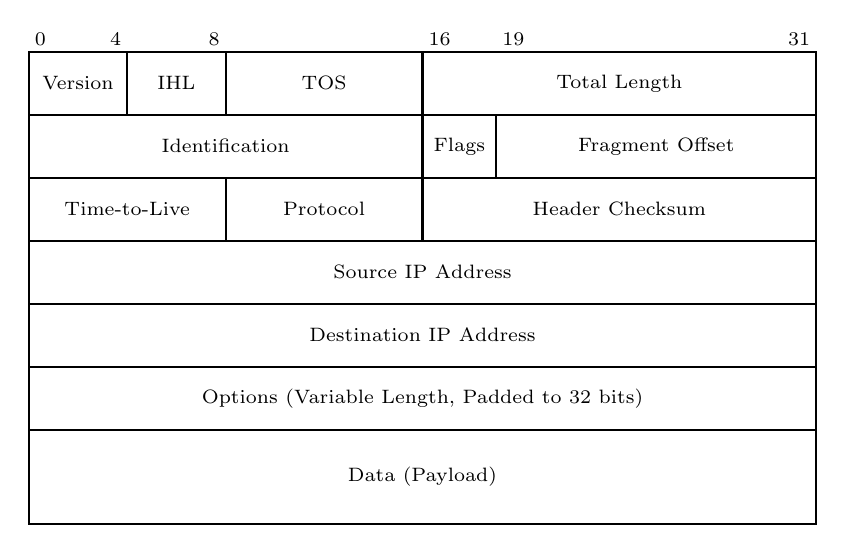
\begin{tikzpicture}[font=\sffamily]
        \def\w{10}
        \def\h{0.8}

        \node[above right, inner sep=2pt, font=\scriptsize] at (0,0) {0};
        \node[above left, inner sep=2pt, font=\scriptsize] at (0.125*\w,0) {4};
        \node[above left, inner sep=2pt, font=\scriptsize] at (0.25*\w,0) {8};
        \node[above right, inner sep=2pt, font=\scriptsize] at (0.5*\w,0) {16};
        \node[above right, inner sep=2pt, font=\scriptsize] at (0.59375*\w,0) {19};
        \node[above left, inner sep=2pt, font=\scriptsize] at (\w,0) {31};

        \draw[thick] (0, 0) rectangle (0.125*\w, -\h) node[midway, font=\scriptsize] {Version};
        \draw[thick] (0.125*\w, 0) rectangle (0.25*\w, -\h) node[midway, font=\scriptsize] {IHL};
        \draw[thick] (0.25*\w, 0) rectangle (0.5*\w, -\h) node[midway, font=\scriptsize] {TOS};
        \draw[thick] (0.5*\w, 0) rectangle (\w, -\h) node[midway, font=\scriptsize] {Total Length};

        \draw[thick] (0, -\h) rectangle (0.5*\w, -2*\h) node[midway, font=\scriptsize] {Identification};
        \draw[thick] (0.5*\w, -\h) rectangle (0.59375*\w, -2*\h) node[midway, font=\scriptsize] {Flags};
        \draw[thick] (0.59375*\w, -\h) rectangle (\w, -2*\h) node[midway, font=\scriptsize] {Fragment Offset};

        \draw[thick] (0, -2*\h) rectangle (0.25*\w, -3*\h) node[midway, font=\scriptsize] {Time-to-Live};
        \draw[thick] (0.25*\w, -2*\h) rectangle (0.5*\w, -3*\h) node[midway, font=\scriptsize] {Protocol};
        \draw[thick] (0.5*\w, -2*\h) rectangle (\w, -3*\h) node[midway, font=\scriptsize] {Header Checksum};

        \draw[thick] (0, -3*\h) rectangle (\w, -4*\h) node[midway, font=\scriptsize] {Source IP Address};

        \draw[thick] (0, -4*\h) rectangle (\w, -5*\h) node[midway, font=\scriptsize] {Destination IP Address};

        \draw[thick] (0, -5*\h) rectangle (\w, -6*\h) node[midway, font=\scriptsize] {Options (Variable Length, Padded to 32 bits)};

        \draw[thick] (0, -6*\h) rectangle (\w, -7.5*\h) node[midway, font=\scriptsize] {Data (Payload)};
    \end{tikzpicture}
    \caption{Detailed Structure of an IPv4 Datagram Header}
    \label{fig:ipv4_datagram}
\end{figure}

\begin{itemize}
    \item \emph{Version number}: A 4-bit field indicating the IP protocol version (e.g., 4 for IPv4).
    \item \emph{Header length (IHL)}: Specifies the length of the header in 32-bit words. Since the minimum header length is 20 bytes, the minimum value of this field is 5. This is a critical field because the options section varies in size.
    \item \emph{Type of service (TOS)}: A sequence of bits intended to determine the priority and handling of the datagram (e.g., low delay or high throughput). In practice, this field was historically underutilized.
    \item \emph{Total length}: A 16-bit field representing the full datagram length (header plus data) in bytes.
    \item \emph{Identifier}: A unique progressive 16-bit number that identifies a datagram, strictly used to assist in the reassembly of fragmented packets.
    \item \emph{Flags and fragmentation offset}: The 3-bit flags field is used to control and identify fragmentation, while the 13-bit \emph{fragmentation offset} specifies where a fragment belongs in the original datagram. The three flag bits are defined as follows \cite{rfc791}:
    \begin{itemize}
        \item \emph{Bit 0}: Reserved; must be strictly zero.
        \item \emph{Bit 1 (Don't Fragment - DF)}: If set to \(1\), routers must not fragment the datagram. If the datagram exceeds the \emph{Maximum Transmission Unit} (MTU) of the next link and cannot be forwarded without fragmentation, it is dropped and an \emph{ICMP error}\footnote{ICMP is a complementary protocol that provides information about delivery failures and routing anomalies. We will describe it more in detail in a dedicated section.} is returned.
        \item \emph{Bit 2 (More Fragments - MF)}: If set to \(1\), it indicates this is not the last fragment. If set to \(0\), it indicates that this is either the last fragment or an unfragmented datagram.
    \end{itemize}
    \item \emph{Time-to-live (TTL)}: A counter decremented by one each time a router processes the datagram. This safeguard ensures that lost or looping packets do not circulate indefinitely across the Internet.
    \item \emph{Protocol}: An 8-bit identifier specifying the upper-layer transport protocol (e.g., TCP or UDP).
    \item \emph{Header checksum}: A mathematical validation sequence applied exclusively to the header fields to detect transmission corruption.
    \item \emph{Options}: An optional, variable-sized metadata field for testing, debugging, and specialized routing. Routers are heavily optimized to process the standard 20-byte IPv4 header.
    The presence of IP options forces the packet to be software-processed, which severely degrades throughput. Consequently, many routers are configured to drop packets with IP options set. In fact, the options field was entirely eliminated in the IPv6 base header.
    \item \emph{Data (Payload)}: The actual variable-size message passed down from the Transport Layer.
\end{itemize}

\subsection{Fragmentation}
When a router receives an IPv4 datagram that is larger than the \emph{Maximum Transmission Unit} (\keyword{MTU}) of the outgoing link, the router must split the packet's payload into smaller pieces to successfully transmit it. This process is known as \keyword{fragmentation} \cite{rfc791}. The router divides the original data and constructs a new IP header for each resulting fragment. To ensure the fragments can be reassembled correctly, the router utilizes specific fields within the IP header: the \emph{identification} field (which remains constant across all fragments of the same datagram), the \emph{flags} field (specifically the \emph{More Fragments} or MF flag), and the \emph{fragment offset} field. 

To minimize the processing overhead on intermediate routers and keep network traffic flowing efficiently, the reassembly of these fragments is strictly delegated to the final receiving end-point. The destination host buffers the incoming fragments and reconstructs the original datagram before passing it up to the transport layer.

\begin{example}{IPv4 Fragmentation}
Suppose a router receives a \(4000\)-byte datagram (consisting of a \(20\)-byte IP header and \(3980\) bytes of data) that must be forwarded across a link with an MTU of \(1500\) bytes. The router will divide the datagram into three fragments:
\begin{itemize}
    \item \emph{Fragment 1:} Carries \(1480\) bytes of data plus a \(20\)-byte header (totaling the \(1500\)-byte MTU). The MF flag is set to \(1\), and the fragment offset is \(0\).
    \item \emph{Fragment 2:} Carries the next \(1480\) bytes of data plus a \(20\)-byte header. The MF flag is set to \(1\), and the fragment offset is \(185\) (calculated as \(1480 / 8\), since offsets are measured in \(8\)-byte blocks).
    \item \emph{Fragment 3:} Carries the remaining \(1020\) bytes of data plus a \(20\)-byte header. The MF flag is set to \(0\) (indicating it is the final fragment), and the fragment offset is \(370\) (\(2960 / 8\)).
\end{itemize}
\end{example}

\subsection{Dynamic Host Configuration Protocol}
The \emph{Dynamic Host Configuration Protocol} (\keyword{DHCP}) is a client-server protocol designed to automatically assign an IP address and other vital network configuration parameters to a new host joining a network \cite{rfc2131}.

Formally, DHCP is classified as an application-layer protocol, even though its primary purpose is to facilitate network-layer connectivity. This classification arises because DHCP communication is built on top of UDP. 

In this architecture, the \emph{client} is the newly connected device requesting network parameters, while the \emph{server} manages a pool of available IP addresses and leases them out. While it is common in residential networks for the DHCP server and the default router (gateway) to be integrated into the exact same physical device, this is not a strict requirement; a DHCP server can operate on a completely separate, dedicated machine.

Adding a new host to the network typically follows a \(4\)-step transaction (often referred to as the DORA process):
\begin{enumerate}
    \item \emph{DHCP Discover}: The new host broadcasts a DHCP discovery message (encapsulated in UDP, targeting destination port \(67\)) to locate a DHCP server. Because the host does not yet have an IP address and does not know the server's address, the message is sent with a source IP of \(0.0.0.0\)\footnote{The \(0.0.0.0\) address is here used to express an unknown IP address.} and a broadcast destination IP of \(255.255.255.255\).
    \item \emph{DHCP Offer}: Because multiple DHCP servers may exist on a network, each server that receives the discovery message and has available addresses responds with a broadcast DHCP offer message (targeting client port \(68\)). This offer includes a proposed IP address, subnet mask, and lease duration.
    \item \emph{DHCP Request}: The new host selects one of the received offers and broadcasts a DHCP request message, echoing the chosen configuration parameters back to the network. This formally accepts the desired lease and implicitly notifies any other responding servers that their offers were declined.
    \item \emph{DHCP ACK}: The selected DHCP server finalizes the binding and transmits a DHCP acknowledgment (ACK) message to the client, officially authorizing the client to begin using the assigned IP address.
\end{enumerate}
 
\subsection{Network Address Translation}
Local network routers act as a primary gateway to the Internet. However, when a specific node on the local network needs to communicate with an external Internet node, exposing its identity poses significant architectural and security challenges. If a local device (such as a network printer) possessed a publicly accessible IP address, any host on the Internet could communicate with it directly. To prevent this security risk, local nodes are assigned private, local IP addresses. Through a technique known as \keyword{IP Masquerading}, the only IP address visible to the external receiving node is the public IP address of the local router.

To route returning traffic back to the correct local node, the router utilizes a \emph{Network Address Translation} (\keyword{NAT}) service \cite{rfc3022}. When the NAT router receives an outbound request from a local node heading to the Internet, it transparently modifies the IP datagram by replacing the private source IP address with its own public gateway IP address. Simultaneously, it modifies the transport-layer packet by replacing the original source port with a \emph{fresh} port number. These fresh ports are dynamically assigned to ensure returning packets can be uniquely mapped back, avoiding routing conflicts when multiple local hosts communicate externally at the same time. Because the packet headers are altered, the NAT router must also meticulously recalculate the IP and TCP/UDP checksums to ensure data integrity. 

The router stores these critical mappings (local IP and port to public IP and fresh port) in a stateful \emph{NAT table}. When the Internet node sends a response, it addresses the packet to the router's public IP and the assigned fresh port. The NAT router intercepts this response, consults its NAT table, reverses the translation by replacing the destination IP and port with the original local IP and port, and forwards the packet inward to the requesting host.

\begin{note}{Architectural Implications of NAT}
The described service is more accurately defined as \emph{Network Address and Port Translation} (\textbf{NAPT}), as it operates on both the IP datagram and the Transport Layer packet. Notably, NAPT breaks the pure end-to-end principle of the ISO/OSI closed architecture. The original design of the Internet assumed that the exact IP address and port leaving a host would arrive unaltered at the destination. By intercepting traffic in the middle and effectively acting as a proxy, NAPT breaks this direct, transparent connection, operating dynamically in the transitional space between Layer 3 and Layer 4.
\end{note}
 
To streamline network configuration and avoid treating arbitrary private IPs as special cases globally, standard bodies have reserved specific blocks of IP addresses exclusively for local network use \cite{rfc1918}. These addresses are non-routable on the public Internet. Key reserved ranges and special addresses include:
\begin{itemize}
    \item \texttt{10.0.0.0 - 10.255.255.255}: Reserved for large private LAN deployments.
    \item \texttt{192.168.0.0 - 192.168.255.255}: Reserved for standard private LAN deployments.
    \item \texttt{127.0.0.0 - 127.255.255.255}: Loopback addresses, used strictly to route traffic back to the host itself.
    \item \texttt{0.0.0.0} (an address with all zeros in the host portion): Used to indicate the network itself or an unknown source address (e.g., during a DHCP Discovery).
    \item \texttt{255.255.255.255} (an address with all ones in the host portion): Used as the limited broadcast address for the local network segment.
\end{itemize}

\section{Internet Control Message Protocol (ICMP)}
The \emph{Internet Control Message Protocol} (\keyword{ICMP}) is a companion protocol to the Internet Protocol (IP). 
While IP is responsible for the routing and delivery of data packets, it lacks built-in mechanisms for error reporting or network diagnostics. 
ICMP bridges this gap by enabling routers and hosts to communicate network-level information, specifically regarding delivery failures and routing anomalies \cite{rfc792}.

Although ICMP is conceptually an integral part of the Network Layer, its messages are not passed directly to the Data Link Layer. 
Instead, ICMP messages are encapsulated within standard IP datagrams with the IP protocol field set to \emph{1}. 
This means ICMP relies on IP for end-to-end delivery, even though it acts as a supervisory protocol for IP itself.

ICMP messages are generally divided into two broad categories: \emph{error-reporting messages} and \emph{query messages}. Each message contains a \emph{type} and a \emph{code} field that specifically identify the nature of the issue or the request. 
Some of the most critical ICMP message types include:

\begin{itemize}
    \item \emph{Destination Unreachable (Type 3)}: Generated by a router or the destination host when a packet cannot be delivered (e.g., due to a missing route, port unavailability, or administrative filtering).
    \item \emph{Time Exceeded (Type 11)}: Sent by a router when it discards a packet because its Time-to-Live (TTL) field has reached zero (\(0\)).
    \item \emph{Echo Request (Type 8) and Echo Reply (Type 0)}: Used to test the reachability of a host across an IP network.
\end{itemize}

The practical utility of ICMP is best illustrated by two network diagnostic utilities:
\begin{itemize}
    \item The \texttt{ping} command relies entirely on ICMP. It sends an ICMP \emph{Echo Request} to a target address and waits for an ICMP \emph{Echo Reply}, allowing the sender to measure the round-trip time and detect packet loss.
    \item The \texttt{traceroute} command exploits the IP TTL field and ICMP error messages. It sends packets (often UDP or ICMP Echo Requests) with sequentially increasing TTL values (\(1, 2, 3, \dots\)). As each packet expires at a successive router along the path, that router returns an ICMP \emph{Time Exceeded} message. By collecting these error messages, the source host can map the entire route to the destination \cite{kurose2017}.
\end{itemize}

\section{IPv6}
To address the imminent exhaustion of IPv4 addresses and to modernize the Internet Protocol, the Internet Engineering Task Force (IETF) standardized \keyword{IPv6} \cite{rfc8200}. The most prominent feature of this new version is its adoption of a \(128\)-bit address space. This ensures that the Internet will effectively never run out of unique IP addresses, allowing for a vast proliferation of connected devices.

\subsection{IPv6 Datagram}
As illustrated in Figure~\ref{fig:ipv6_datagram}, beyond its expanded address capacity, IPv6 introduces a streamlined, fixed-size \(40\)-byte base header. 
This redesign deliberately eliminates several IPv4 fields --- such as fragmentation offsets and the header checksum --- to significantly reduce processing overhead at intermediate routers.

\begin{figure}[htbp]
    \centering
    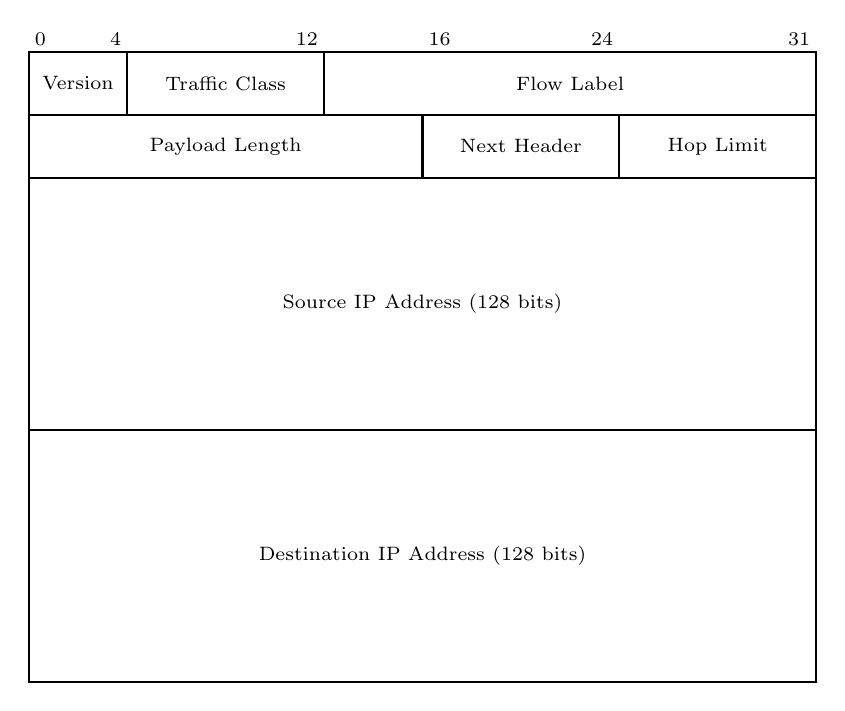
\begin{tikzpicture}[font=\sffamily]
        \def\w{10}
        \def\h{0.8}

        \node[above right, inner sep=2pt, font=\scriptsize] at (0,0) {0};
        \node[above left, inner sep=2pt, font=\scriptsize] at (0.125*\w,0) {4};
        \node[above left, inner sep=2pt, font=\scriptsize] at (0.375*\w,0) {12};
        \node[above right, inner sep=2pt, font=\scriptsize] at (0.5*\w,0) {16};
        \node[above left, inner sep=2pt, font=\scriptsize] at (0.75*\w,0) {24};
        \node[above left, inner sep=2pt, font=\scriptsize] at (\w,0) {31};

        \draw[thick] (0, 0) rectangle (0.125*\w, -\h) node[midway, font=\scriptsize] {Version};
        \draw[thick] (0.125*\w, 0) rectangle (0.375*\w, -\h) node[midway, font=\scriptsize] {Traffic Class};
        \draw[thick] (0.375*\w, 0) rectangle (\w, -\h) node[midway, font=\scriptsize] {Flow Label};

        \draw[thick] (0, -\h) rectangle (0.5*\w, -2*\h) node[midway, font=\scriptsize] {Payload Length};
        \draw[thick] (0.5*\w, -\h) rectangle (0.75*\w, -2*\h) node[midway, font=\scriptsize] {Next Header};
        \draw[thick] (0.75*\w, -\h) rectangle (\w, -2*\h) node[midway, font=\scriptsize] {Hop Limit};

        \draw[thick] (0, -2*\h) rectangle (\w, -6*\h) node[midway, font=\scriptsize] {Source IP Address (128 bits)};

        \draw[thick] (0, -6*\h) rectangle (\w, -10*\h) node[midway, font=\scriptsize] {Destination IP Address (128 bits)};
    \end{tikzpicture}
    \caption{Detailed Structure of an IPv6 Datagram Header}
    \label{fig:ipv6_datagram}
\end{figure}

The individual fields of the IPv6 header operate as follows:

\begin{itemize}
    \item \emph{Version} (\(4\) bits): Contains the fixed value of \(6\), which identifies the packet as an IPv6 datagram.
    \item \emph{Traffic Class} (\(8\) bits): Functionally equivalent to the IPv4 Type of Service (ToS) field. It is used by originating nodes and forwarding routers to identify and distinguish between different classes or priorities of IPv6 packets, facilitating Quality of Service (QoS) \cite{rfc8200}.
    \item \emph{Flow Label} (\(20\) bits): A novel addition in IPv6, this field allows a source to label sequences of packets (flows) that require special handling by routers, such as non-default QoS or real-time service routing constraints \cite{rfc6437}.
    \item \emph{Payload Length} (\(16\) bits): Specifies the size of the packet payload in bytes, encompassing any \emph{extension headers} and the upper-layer protocol data. Unlike the IPv4 \emph{Total Length} field, this value does not include the size of the base IPv6 header itself since IPv6 headers have fixed size of \(40\)-byte.
    \item \emph{Next Header} (\(8\) bits): Replacing the IPv4 \emph{Protocol} field, this dictates the type of header immediately following the base IPv6 header. This modular design natively supports the chaining of \keyword{extension headers}, allowing optional network-layer information to be processed only at the destination node rather than at every hop along the path.
    \item \emph{Hop Limit} (\(8\) bits): Renames the IPv4 \emph{Time-to-Live} (TTL) field.
    \item \emph{Source IP Address} (\(128\) bits): The address of the packet's initial sender.
    \item \emph{Destination IP Address} (\(128\) bits): The address of the packet's intended recipient (which may not be the ultimate destination if a Routing Extension Header is present).
\end{itemize}

Unlike IPv4, the IPv6 base header completely lacks a checksum field. This architectural decision delegates error detection to the link layer (e.g., Ethernet CRC) and upper-layer transport protocols (e.g., TCP or UDP).
In IPv4, due to to the TTL field decrementing, each router would recalculate the checksum. This design choice hence guarantees a faster packet forwarding.

The \(16\)-bit \emph{Payload Length} field restricts standard IPv6 payloads to \(65,535\) bytes. However, if an application requires transferring a larger payload in a single packet, IPv6 accommodates this by setting the Payload Length field to \(0\) and utilizing a Hop-by-Hop \keyword{Jumbo Payload} extension header \cite{rfc2675}. This capability enables payloads up to \(4,294,967,295\) bytes in length, heavily optimizing throughput on high-capacity links.

Another crucial difference lies in how packet fragmentation is handled. In IPv4, intermediate routers can fragment packets that exceed the MTU of the outgoing link. 
Conversely, IPv6 shifts this responsibility entirely to the source node \cite{rfc8200}. If a router receives an IPv6 packet that is too large for the next hop, it discards the packet and returns an ICMPv6 \q{Packet Too Big} message, prompting the source to perform \keyword{Path MTU Discovery} (PMTUD) \cite{rfc8201}.
Because intermediate routers no longer perform fragmentation, endpoints must correctly implement PMTUD to avoid having packets dropped. 

\begin{note}{}
    If an endpoint's firewall improperly drops inbound ICMPv6 \q{Packet Too Big} messages, communication across networks with smaller MTUs will silently fail.
\end{note}

Furthermore, IPv6 completely eliminates the broadcast addressing method used in IPv4, relying entirely on more robust and targeted multicast and anycast mechanisms. 
It also introduces the \emph{Neighbor Discovery Protocol} (\keyword{NDP}), which implements some of the features implemented by the \emph{Address Resolution Protocol} (ARP) -- we will talk about it in the next chapter -- in the legacy TCP/IP stack and operates securely and efficiently over ICMPv6 \cite{rfc4861}.

\begin{observation}{What about IPv5?}
    Given the leap from IPv4 to IPv6, a common question is what happened to IPv5. The version number \(5\) was historically allocated to the \emph{Internet Stream Protocol} (ST, and its successor ST-II) \cite{rfc1819}. This was an experimental protocol designed in the late 1970s and 1990s to provide connection-oriented, guaranteed-bandwidth streams for real-time voice and video transmission. Because it already used the IP version number \(5\) in its packet headers, the next-generation Internet Protocol was naturally designated as IPv6 to avoid any conflict. ST-II never saw widespread public deployment.
\end{observation}

\section{Best-effort Networks}

When transmitting data across a network, the network layer theoretically could offer a variety of delivery services to the transport layer. These potential services include:
\begin{itemize}
    \item \emph{Guaranteed delivery:} Ensuring every packet reaches its destination.
    \item \emph{Guaranteed delivery within a bounded delay:} Ensuring packets arrive within a strict timeframe, which is critical for real-time applications.
    \item \emph{In-order packet delivery:} Ensuring that packets arrive in the exact sequence they were transmitted.
    \item \emph{Guaranteed minimal bandwidth:} Reserving a specific data rate for a flow.
    \item \emph{Security:} Providing built-in encryption or authentication at the network layer.
\end{itemize}

In practice, however, standard IP networks offer absolutely none of these guarantees. The core architectural philosophy of the Internet relies on a \keyword{best-effort service} \cite{kurose2017}. This means the network simply tries its best to deliver a packet from the source to the destination, but it promises nothing regarding reliability, ordering, timing, or bandwidth. 

Empirically, this stripped-down, best-effort network layer design, when combined with adequately provisioned bandwidth and intelligent transport-layer protocols (like TCP) operating at the network edges, has proven to be incredibly resilient, scalable, and fully adequate for the vast majority of modern applications.

\section{Routers}

A \keyword{router} is a specialized network device equipped with multiple incoming and outgoing communication links. Its fundamental responsibility is to move data across the network toward its final destination. This overarching responsibility is divided into two distinct but related functions:
\begin{itemize}
    \item \emph{Forwarding:} The localized, microscopic action of moving a packet from a specific input link to the correct output link. The passage of a message from one router to an adjacent router is commonly referred to as a \emph{hop}.
    \item \emph{Routing:} The network-wide, macroscopic process of determining the end-to-end path that packets should take from source to destination. The router must know this path, but as network architectures evolve, the router itself does not necessarily have to compute it locally.
\end{itemize}

To perform forwarding, each router maintains a \emph{forwarding table}—a data structure that maps destination IP address prefixes to specific output links. These tables can be constructed using two primary paradigms:
\begin{itemize}
    \item \emph{Decentralized:} Each router runs routing algorithms and builds its forwarding table by actively communicating and exchanging route information with other routers.
    \item \emph{Centralized:} A central remote controller logically computes the routing paths via software and distributes the resulting forwarding tables to the routers. This paradigm is known as \emph{Software-Defined Networking} (SDN).
\end{itemize}

Strictly speaking, a router's primary packet-processing job ends within the \emph{Network Layer} (Layer 3 of the OSI model). However, most modern commercial routers implement the entire network stack to support complex management interfaces (like SSH or web servers), security features, and diagnostic tools.

\subsection{Logical Architecture}
A modern router is composed of several distinct logical components \cite{kurose2017}:

\begin{figure}[htbp]
    \centering
    \begin{tikzpicture}[
        >=stealth,
        node distance=1.5cm and 2cm,
        port/.style={draw, rectangle, minimum height=1.2cm, minimum width=2.5cm, align=center, font=\small},
        buffer/.style={draw, rectangle, minimum height=0.4cm, minimum width=0.7cm, align=center, fill=orange!5, font=\footnotesize},
        fabric/.style={draw, circle, minimum width=3cm, align=center, fill=gray!10, font=\bfseries},
        proc/.style={draw, rectangle, rounded corners, minimum height=1.0cm, minimum width=3.5cm, align=center, fill=blue!5, font=\small},
        table/.style={draw, rectangle, minimum height=1cm, minimum width=3.2cm, align=center, fill=blue!2, font=\small}
    ]
    
    \node[fabric] (switch) at (0,0) {Switch\\Fabric};
    \node[table, above=0.6cm of switch] (ftable) {Forwarding Table};
    \node[proc, above=0.6cm of ftable] (processor) {Routing Processor};
    
    \node[port] (port1) at (150:4cm) {Port};
    \node[port] (port2) at (210:4cm) {Port};
    \node[port] (port3) at (270:4cm) {Port};
    \node[port] (port4) at (330:4cm) {Port};
    \node[port] (port5) at (30:4cm)  {Port};

    \node[buffer, anchor=north east, xshift=0.1cm, yshift=0.1cm] (buf1) at (port1.north east) {Buffer};
    \node[buffer, anchor=south east, xshift=0.1cm, yshift=-0.1cm] (buf2) at (port2.south east) {Buffer};
    \node[buffer, anchor=south east, xshift=0.1cm, yshift=-0.1cm] (buf3) at (port3.south east) {Buffer};
    \node[buffer, anchor=north east, xshift=0.1cm, yshift=0.1cm] (buf4) at (port4.north east) {Buffer};
    \node[buffer, anchor=south east, xshift=0.1cm, yshift=-0.1cm] (buf5) at (port5.south east) {Buffer};

    \draw[<->, thick] (port1) -- (switch);
    \draw[<->, thick] (port2) -- (switch);
    \draw[<->, thick] (port3) -- (switch);
    \draw[<->, thick] (port4) -- (switch);
    \draw[<->, thick] (port5) -- (switch);
    
    \draw[-, dashed] (processor) -- (ftable);
    \draw[-, dashed] (ftable) -- (switch);
    
    \draw[-, thick] (port1.150) -- ++(150:1.5cm) node[midway, above, sloped, font=\scriptsize] {Link};
    \draw[-, thick] (port2.210) -- ++(210:1.5cm) node[midway, above, sloped, font=\scriptsize] {Link};
    \draw[-, thick] (port3.270) -- ++(270:1.5cm) node[midway, above, sloped, font=\scriptsize] {Link};
    \draw[-, thick] (port4.330) -- ++(330:1.5cm) node[midway, above, sloped, font=\scriptsize] {Link};
    \draw[-, thick] (port5.30)  -- ++(30:1.5cm)  node[midway, above, sloped, font=\scriptsize] {Link};

    \end{tikzpicture}
    \caption{Logical Architecture of a Router. Each port is both an input and an output port, depending on the specific data flow.}
    \label{fig:router_architecture}
\end{figure}

\begin{itemize}
    \item \emph{Input ports:} These are the physical input interfaces for incoming links. When a packet arrives, the input port parses the destination IP address and consults a localized copy of the forwarding table to decide the appropriate output port. Because routing tables use address prefixes, an IP address might match multiple entries; the router resolves this using a \emph{longest prefix match} algorithm to select the most specific route. The packet is then sent into the switch fabric.
    \item \emph{Switch fabric:} This is the internal heart of the router, connecting input ports to output ports. The switch fabric can be implemented in several ways, each with distinct performance implications:
    \begin{itemize}
        \item \emph{Via memory:} The simplest approach, where an internal CPU copies the packet from the input port to memory, and then to the output port. This is slow and limits the router's throughput to the memory bandwidth.
        \item \emph{Via bus:} Packets are sent over a shared internal bus. This is hardware-accelerated but only one packet can traverse the bus at a time, leading to serialization delays.
        \item \emph{Via interconnection network (crossbar):} A complex grid of physical switches allows multiple packets from different input ports to be forwarded to different output ports simultaneously. This is the fastest and most scalable architecture.
    \end{itemize}
    \item \emph{Routing processor:} The CPU that runs the routing protocols, computes the routing tables (in a decentralized setup), or communicates with the remote SDN controller (in a centralized setup).
    \item \emph{Output ports:} The physical ports that transmit the packets onto the outgoing links.
    \item \emph{Buffers:} Because internal switching or packet arrival rates can temporarily exceed the outgoing link's transmission speed, packets are stored in buffers. To manage these queues, routers employ \emph{schedulers} (such as First-Come-First-Serve, Priority Queuing, or Round-Robin) and implement active queue management to decide which packets should be dropped if the buffer becomes entirely full.
\end{itemize}

It is worth noting that physical interfaces on a router are typically bidirectional line cards; thus, the same physical module acts simultaneously as an input port and an output port depending on the direction of the traffic flow.

\subsection{Routing}
Routing algorithms can broadly be classified into two main paradigms based on how they process information to determine network paths \cite{kurose2017}:
\begin{itemize}
    \item \keyword{Centralized routing}: The path computation is handled with global knowledge of the network. This can be \emph{logically centralized}, where each router possesses a complete graph representation of the network topology and computes routes locally, or \emph{physically centralized}, where a dedicated control node (e.g., a Software-Defined Networking controller) calculates the routes and updates the forwarding tables of all routers.
    \item \keyword{Decentralized routing}: Both logically and physically decentralized. In this approach, routers compute paths iteratively by communicating exclusively with their physically adjacent peers. No single router possesses the complete representation of the network graph.
\end{itemize}

\subsubsection{Flooding}
The simplest approach to packet forwarding is \keyword{flooding}. In this mechanism, each router forwards an incoming message on all of its outgoing links, except the one from which the message arrived. 

While conceptually trivial, flooding causes the number of messages to grow exponentially, assuming the average node degree is greater than two. In large-scale networks, this leads to immense broadcast storms, making the approach highly impractical for standard data routing. However, flooding is extremely robust; because copies of the message travel along all possible paths, it is guaranteed that at least one copy will traverse the optimal path. This makes it suitable for scenarios where high redundancy and fault tolerance are critical, such as military networks or network knowledge distribution between routers.

\subsubsection{Distance-Vector (DV)}
The \keyword{Distance-Vector} algorithm is a decentralized routing protocol heavily reliant on the Bellman-Ford algorithm \cite{kurose2017}. Each router maintains a vector containing its estimated shortest distances to all other nodes in the network. 

The optimal path is calculated iteratively using the Bellman-Ford equation. Let \(x\) be the computing node, \(y\) be the destination, and \(\alpha\) represent a directly connected neighbor of \(x\). The minimum distance \(d_x[y]\) is calculated as:
\[ d_x[y] = \min_{\alpha \in N(x)}\set{c(x, \alpha) + d_{\alpha}[y]} \]
where \(c(x, \alpha)\) is the link cost from \(x\) to \(\alpha\), and \(N(x)\) is the set of \(x\)'s neighbors.

The execution flow of the Distance-Vector algorithm follows these steps \cite{rfc2453}:
\begin{enumerate}
    \item \emph{Initialization}: Node \(x\) initializes the distance to itself as 0. For each neighbor \(v\), the distance \(d_x[v]\) is set to the direct link cost \(c(x, v)\). For all non-neighbor destinations, the distance is initialized to \(\infty\).
    \item \emph{Neighbor State Initialization}: Node \(x\) allocates space for the distance vectors of its neighbors, initializing their distances to unknown values. The router stores these distance vectors in a data structure usually known as \keyword{routing table}, not to be confused with the \emph{forwarding table}\footnote{The forwarding table is directly derived from routing table and contains the fastest IP-router associations.}.
    \item \emph{Advertisement}: Node \(x\) sends its initialized distance vector to all adjacent neighbors.
    \item \emph{Active Execution}: Node \(x\) enters a loop where it listens for updates from neighbors. Upon receiving an update, it recalculates its distances using the Bellman-Ford equation. If any distance \(d_x[v]\) changes (where negative costs are strictly disallowed), \(x\) transmits its updated vector to its neighbors.
\end{enumerate}

This algorithm has a worst-case computational complexity of \(O(\abs{N} \cdot \abs{E})\) during convergence, as every node potentially updates its paths based on traversing all network edges.

The DV algorithm operates asynchronously. Updates occur in a non-blocking fashion, meaning that routers do not need to pause their normal forwarding operations or operate in lockstep. This allows for continuous data forwarding while the routing protocol independently converges in the background.

\subsubsection{Vulnerabilities of Distance-Vector}
Because a node fundamentally trusts the routing information provided by its neighbors (often described as \qi{routing by rumor}), the DV algorithm is susceptible to several critical issues.

\paragraph{Count-to-Infinity}
Consider a linear network topology: \( A \) --- \( B \) --- \( C \), where both links have a cost of 1. Initially, \( A \) routes to \( C \) via \( B \) with a total cost of 2, and \( B \) routes to \( C \) with a cost of 1. 

If the link between \( B \) and \( C \) suddenly fails, \( B \) detects the failure and updates its direct cost to \( C \) as \( \infty \). However, before \( B \) can advertise this failure, it might receive a periodic update from \( A \) claiming a distance of 2 to \( C \). \( B \), unaware that \( A \)'s path goes through \( B \) itself, incorrectly assumes it can reach \( C \) via \( A \) with a cost of \( 1 + 2 = 3 \). \( B \) updates its table and informs \( A \). \( A \) then updates its distance to \( 1 + 3 = 4 \). This feedback loop continues indefinitely, incrementing the costs to infinity \cite{tanenbaum2011}.

\paragraph{Crazy Router}
If a malfunctioning or malicious router advertises a distance of 0 to all destinations in the network, it establishes itself as the lowest-cost path for all traffic. The compromised router will attract an overwhelming amount of network traffic, likely causing the router to soon become unavailable. 
Given the count-to-infinity problem and slow convergence, the network will persistently forward packets into this \qi{black hole} long after the router crashes under the load.

\vspace{2mm}
To mitigate routing loops and the count-to-infinity problem, implementations often use the \keyword{poisoned reverse} technique, that dictates that if node \(A\) routes to destination \(C\) through node \(B\), \(A\) will falsely advertise to \(B\) that its distance to \(C\) is \(\infty\). By doing so, \(B\) will never attempt to route traffic to \(C\) backward through \(A\), effectively severing two-node loops \cite{rfc2453}.

\subsubsection{Link-State (LS)}
In contrast to the Distance-Vector approach, the \keyword{Link-State} algorithm relies on global network topology distribution \cite{rfc2328}. Every node broadcasts Link-State Packets (LSPs) that contain its identifier and the exact costs of its directly attached links.

The operation follows a distinct five-step procedure:
\begin{enumerate}
    \item \emph{Neighbors' Discovery}: A router transmits a short HELLO packet across all active interfaces. Connected neighbors respond, exchanging their unique IDs.
    \item \emph{Costs Setup}: The router measures or assigns the communication cost (e.g., delay, bandwidth metric) to each of its discovered neighbors.
    \item \emph{Packet Construction}: The router generates an LSP encapsulating its ID, the list of its immediate neighbors, the measured link costs, and a sequence number.
    \item \emph{Packets Exchange}: The router floods this packet to all other nodes in the entire network. Through this reliable broadcast mechanism, every router eventually receives an identical set of LSPs, allowing each node to independently map the exact topology of the network.
    \item \emph{Dijkstra Computation}: Armed with the complete network graph, each router locally executes Dijkstra's Algorithm to compute the shortest-path tree from itself to all other destinations.
\end{enumerate}

Unlike DV, the Link-State algorithm exhibits a more synchronous initialization behavior. Before a newly booted node can safely begin computing optimal routes and forwarding external traffic, it must wait to receive the LSPs from the network to construct a complete and accurate topological map.

